\documentclass{article}
\usepackage[utf8]{inputenc}

\title{MATH3160 — Portfolio 4.2}
\author{Mike Medved}
\date{October 8th, 2022}

\usepackage{color}
\usepackage{amsthm}
\usepackage{amssymb} 
\usepackage{amsmath}
\usepackage[margin=1in]{geometry} 
\usepackage{listings}
\usepackage[dvipsnames]{xcolor}
\usepackage{tikz}

\begin{document}

\maketitle

\section{Deliverables}

\subsection{Tools for Discrete Random Variables}

The following are a few of the available tools to work with discrete random variables.

\subsubsection{Probability Mass Function (pmf)}

The probability mass function, or \textit{pmf} for short is a function that maps a discrete random variable to its probability. The pmf is in the domain of the image of the random variable $X$ and the range of the probability.

$$
f(x) = P(X = x)
$$

$\hfill \break$
Further, the sum of all pmf of $X$ must be equal to one in order to satisfy the law of total probability:

$$
\sum_{x \in \textit{Im(X)}} f(x) = 1
$$

\subsubsection{Cumulative Distribution Function (cdf)}

The cumulative distribution function, or \textit{cdf} for short is a function that maps a discrete random variable to its cumulative probability. The cdf is in the domain of the image of the random variable $X$ and the range of the cumulative probability.

$$
F(x) = P(X \leq x)
$$

\subsubsection{Example of 1.1.1 and 1.1.2}

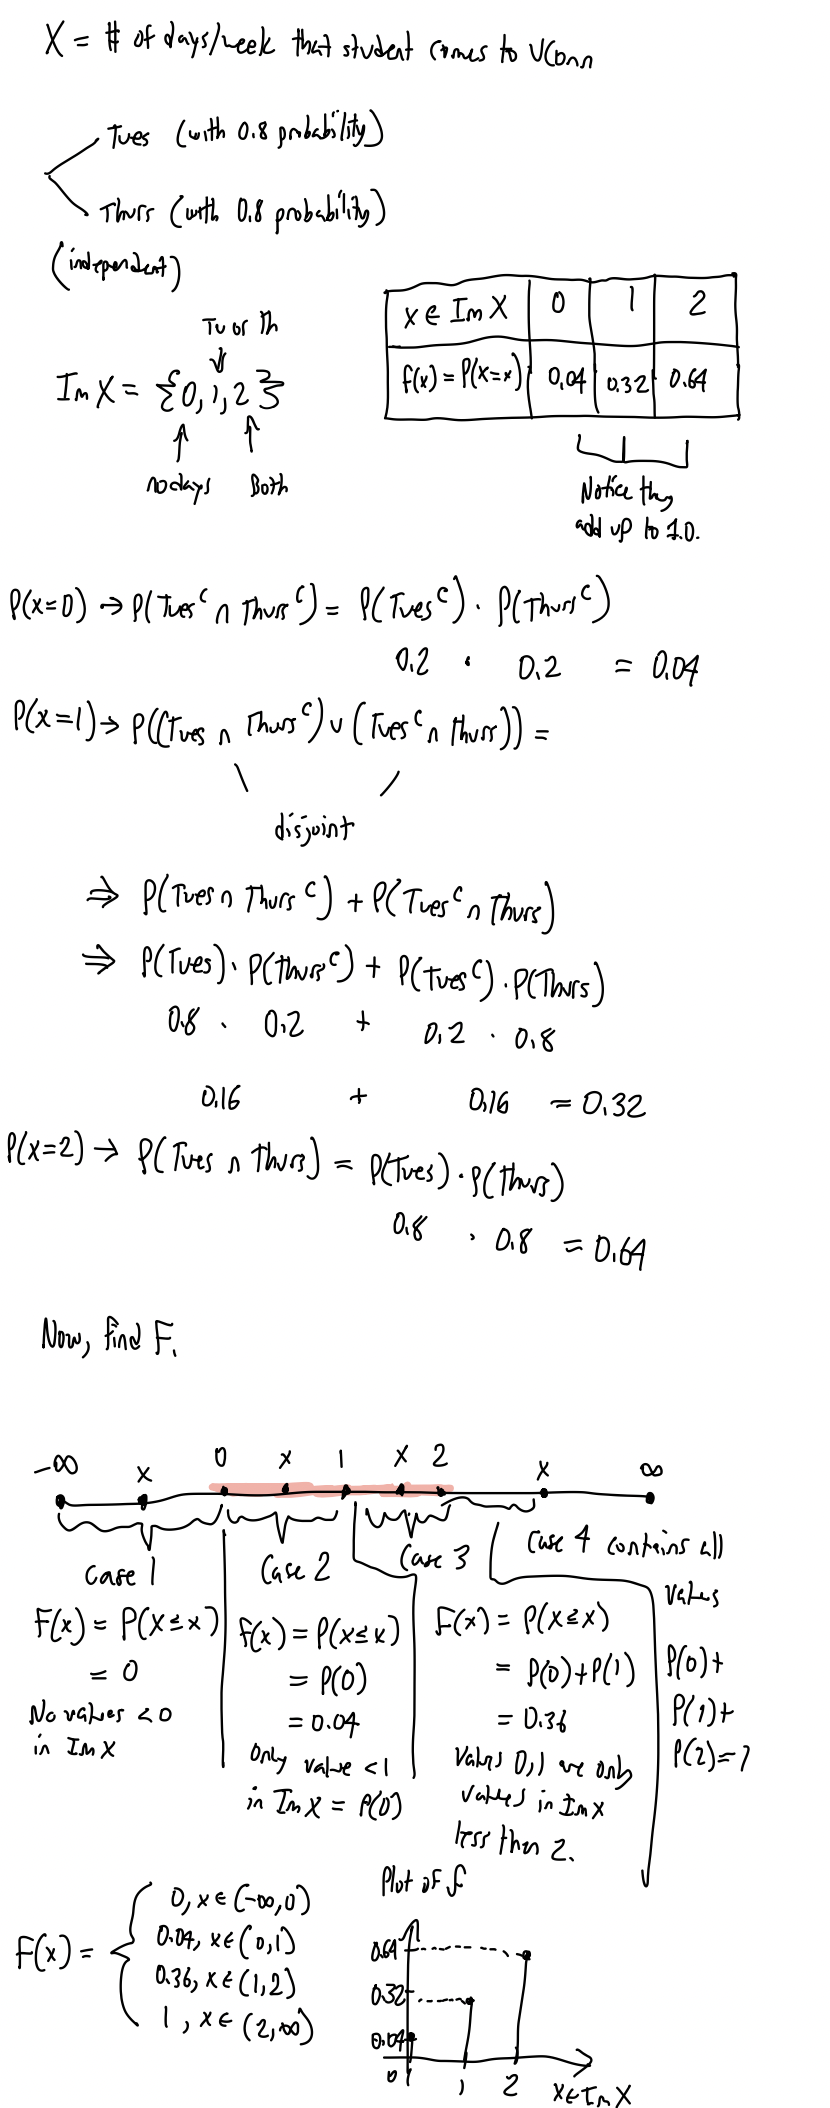
\includegraphics[height=9in]{example-pmf-cdf.png}

\subsubsection{Expectation}

The expectation of a discrete random variable $X$ is the weighted average of the random variable.

$$
E\left[X\right] = \sum_{x \in \textit{Im(X)}} x \cdot P(X = x)
$$

$\hfill \break$
The intuition behind the expectation of $X$, is that it is the value around which we \textit{expect} the random variable $X$ to be situated.

\subsubsection{Variance}

The variance of a discrete random variable $X$ is the weighted average of the squared deviation of the random variable from its expectation.

$$
\textit{Var}(X) = E\left[\left(X-E\left[X\right]^2\right)\right]
$$

$\hfill \break$
The intuition behind the variance of $X$, is that it is the average spread/deviation of the possible values of $X$ around the expectation $E\left[X\right]$.

\subsubsection{Example of 1.1.4 and 1.1.5}

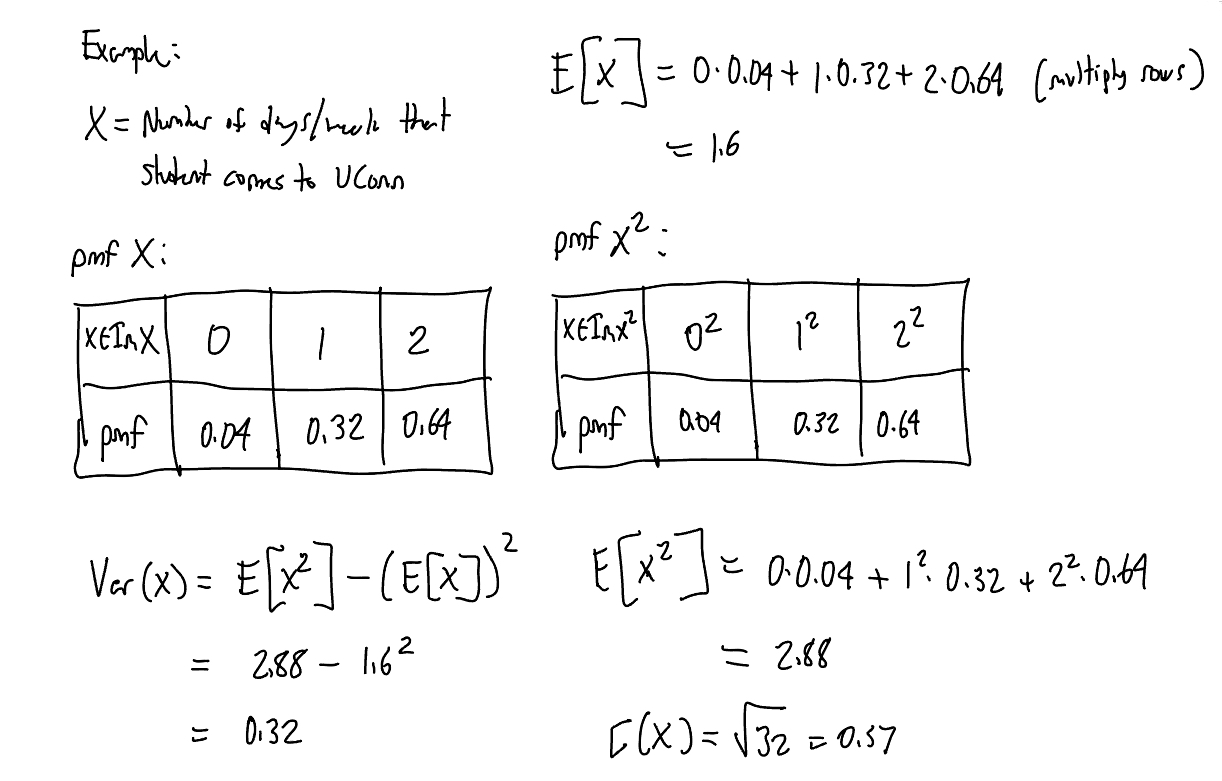
\includegraphics[height=4.25in]{example-expect-var.jpeg}

\newpage
\subsubsection{Properties of Expectation and Variance}

There are several important properties that the expectation and variance functions hold:

\begin{enumerate}
    \item The expectation of a constant is that constant, $E\left[C\right] = C$.
    \item The expectation of a random variable $X$ must be positive, $E\left[X\right] \geq 0$.
    \item The sum of two random variables is the sum of their expectations, $E\left[aX + bY\right] = a \cdot E\left[X\right] + b \cdot E\left[Y\right]$.
    \begin{itemize}
        \item If $a, b = 1$: $E\left[X+Y\right] = E\left[X\right] + E\left[Y\right]$.
    \end{itemize}
    \item If $X \leq Y$, then the expectations follow this property, $E\left[X\right] \leq E\left[Y\right]$.
    \item The product of two expectations does not equal the individual products, $E\left[X \cdot Y\right] \neq E\left[X\right] \cdot E\left[Y\right]$.
    \begin{itemize}
        \item The only exception to this property is if $X$ and $Y$ are independent, then the product of the expectations \textit{is} equal to the individual products, $E\left[X \cdot Y\right] = E\left[X\right] \cdot E\left[Y\right]$.
    \end{itemize}
    \item The transport formula reveals the process of transferring a random variable into a normal variable:
    $$
    E\left[g(X)\right] = \sum_{x \in \textit{Im(X)}} g(x) \cdot P(X = x)
    $$
    $\hfill \break$
    The composition between a random variable $X$ and a real function $g$ is a random variable $g(X)$.
    \item Generally, the variance of the sum of two random variables, does not equal the sum of it's individual components, $\textit{Var(X+Y)} \neq \textit{Var(X)} + \textit{Var(Y)}$.
    \begin{itemize}
        \item Similarly to the product of two expectations, the only exception to this property is if $X$ and $Y$ are independent, then the sum of the variances \textit{is} equal to the individual sums such that, $\textit{Var(X+Y)} = \textit{Var(X)} + \textit{Var(Y)}$.
    \end{itemize}
\end{enumerate}

\end{document}